\documentclass[aspectratio=169]{beamer}

\usetheme{CERN}

\beamertemplatenavigationsymbolsempty

\usepackage{graphicx}
\usepackage{booktabs}

\usepackage{xcolor}
\usepackage{graphicx}
\usepackage{multicol}
\usepackage{wrapfig}

\graphicspath{ {images/} }
\usepackage[export]{adjustbox}

%----------------------------------------------------------------------------------------
%	TITLE PAGE
%----------------------------------------------------------------------------------------

\title[Configuration Management @ CERN]{Configuration Management @ CERN\\
        *Going Agile with Style}
\author{Andrea Giardini}
\date{\today}

\institute[CERN]
{
CERN \\
\medskip
\textit{andrea.giardini@cern.ch}
}
\date{24 April 2015 - PuppetCamp Berlin}


\begin{document}

\cernSplashBlue

\begin{frame}
\titlepage
\end{frame}

\begin{frame}
\frametitle{Outline}
\tableofcontents
\end{frame}

%------------------------------------------------
%	PRESENTATION SLIDES
%------------------------------------------------

%------------------------------------------------
\section{Introduction}
%------------------------------------------------

\subsection{What is CERN}

\begin{frame}

    \frametitle{What is CERN}
    \begin{minipage}[t]{0.95\textwidth}
        \begin{columns}
            \begin{column}{0.5\textwidth}
                \begin{itemize}
                    \item European Organization for Nuclear Research
                    \item Situated in the border between Switzerland and France
                    \item 21 Member states
                    \item Big challenges 
                \end{itemize}
            \end{column}
            \begin{column}{0.5\textwidth}
                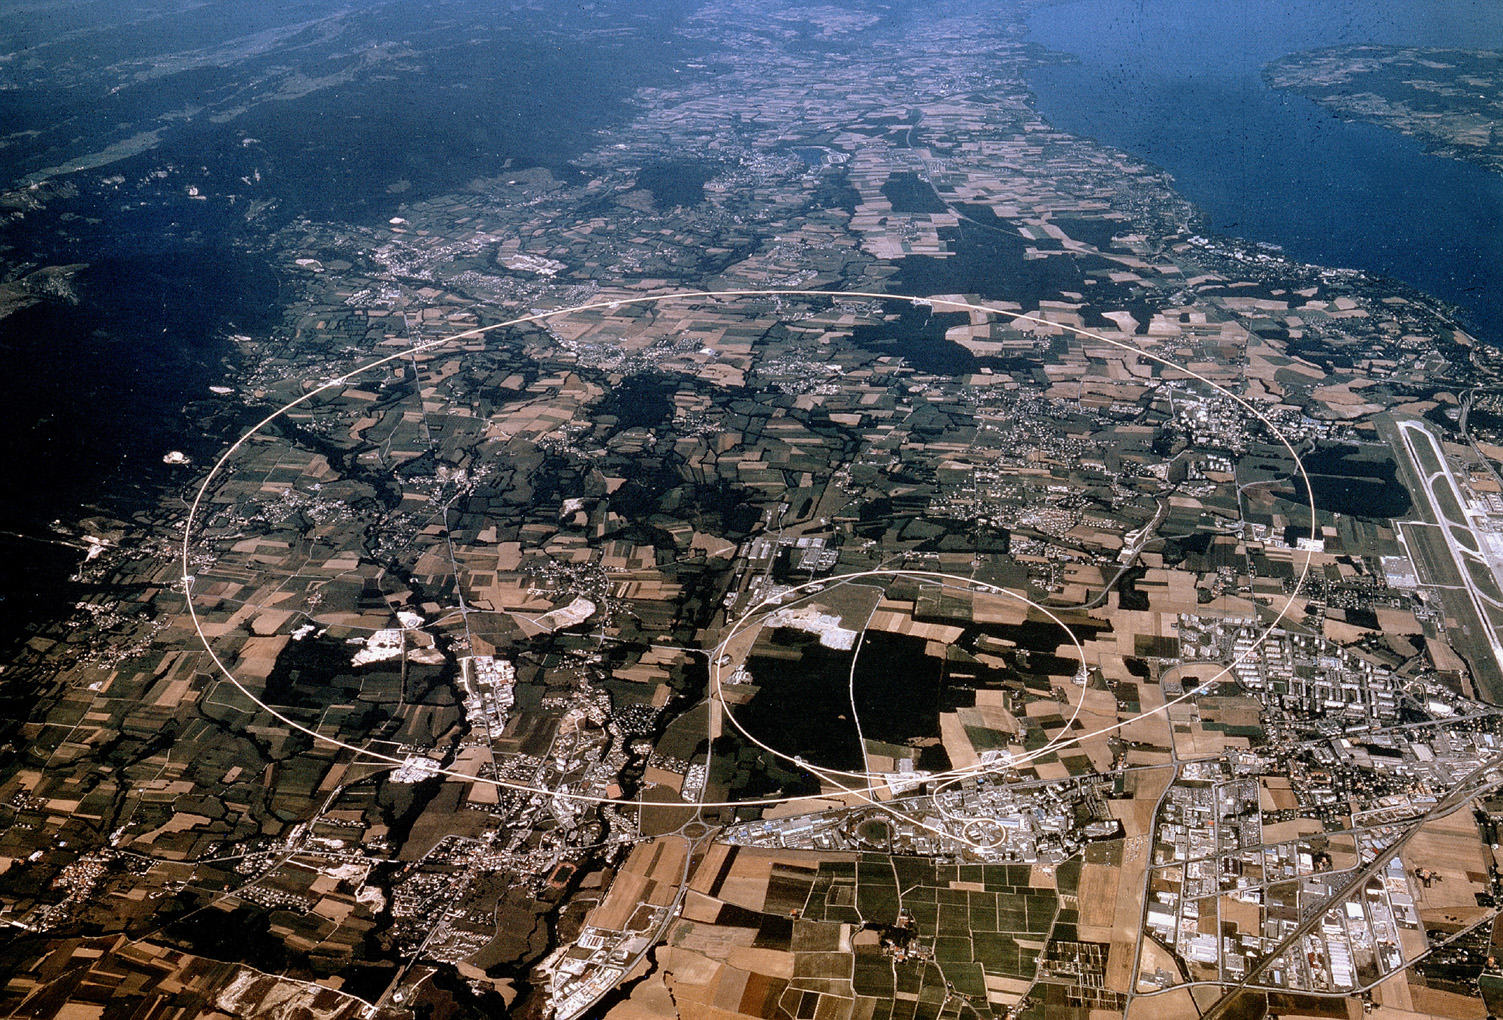
\includegraphics[width=1.1\textwidth]{CernMap.jpg}
            \end{column}
        \end{columns}
    \end{minipage}

\end{frame}

%------------------------------------------------

\begin{frame}
    \frametitle{Big Challenges - The FCC}
    \begin{center}
        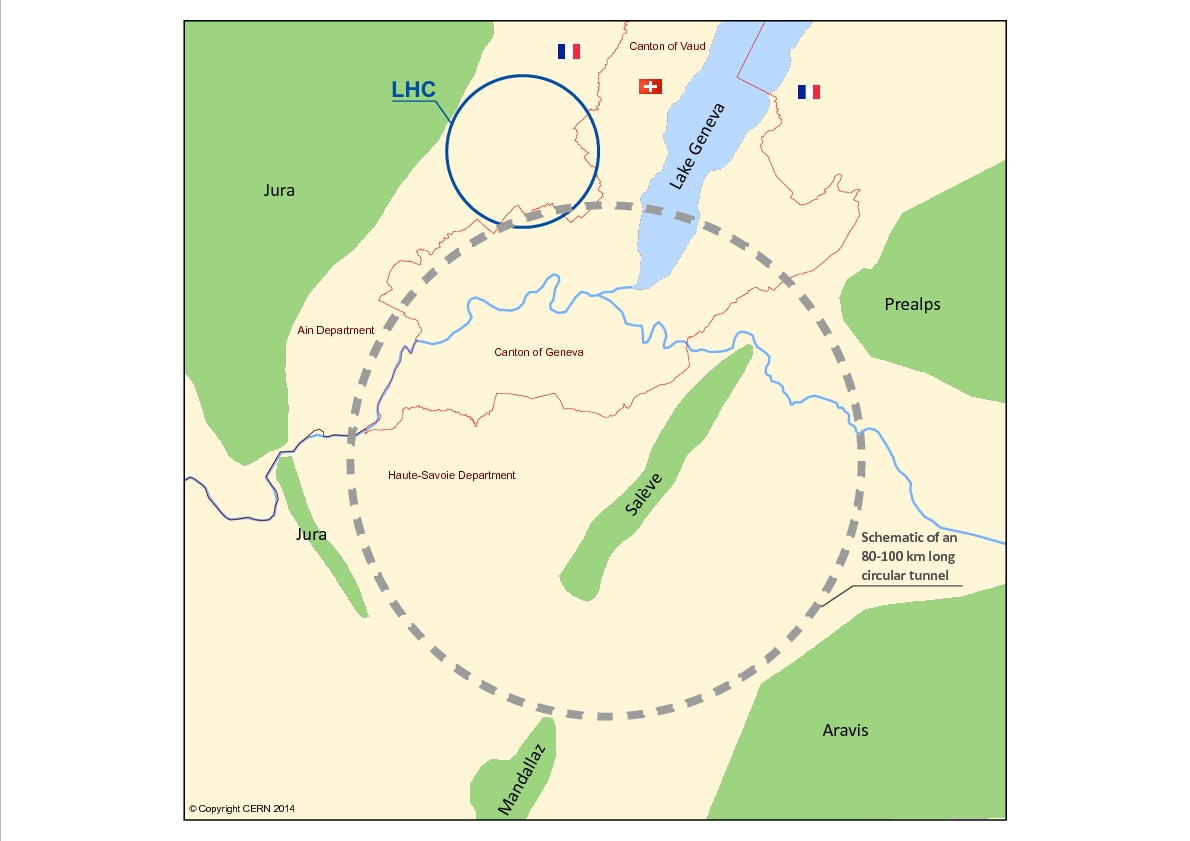
\includegraphics[width=0.65\textwidth,trim=4 4 4 4,clip]{CERN_LCC.jpg}
    \end{center}
\end{frame}

%------------------------------------------------

\begin{frame}
    \frametitle{The LHC}
    \begin{center}
        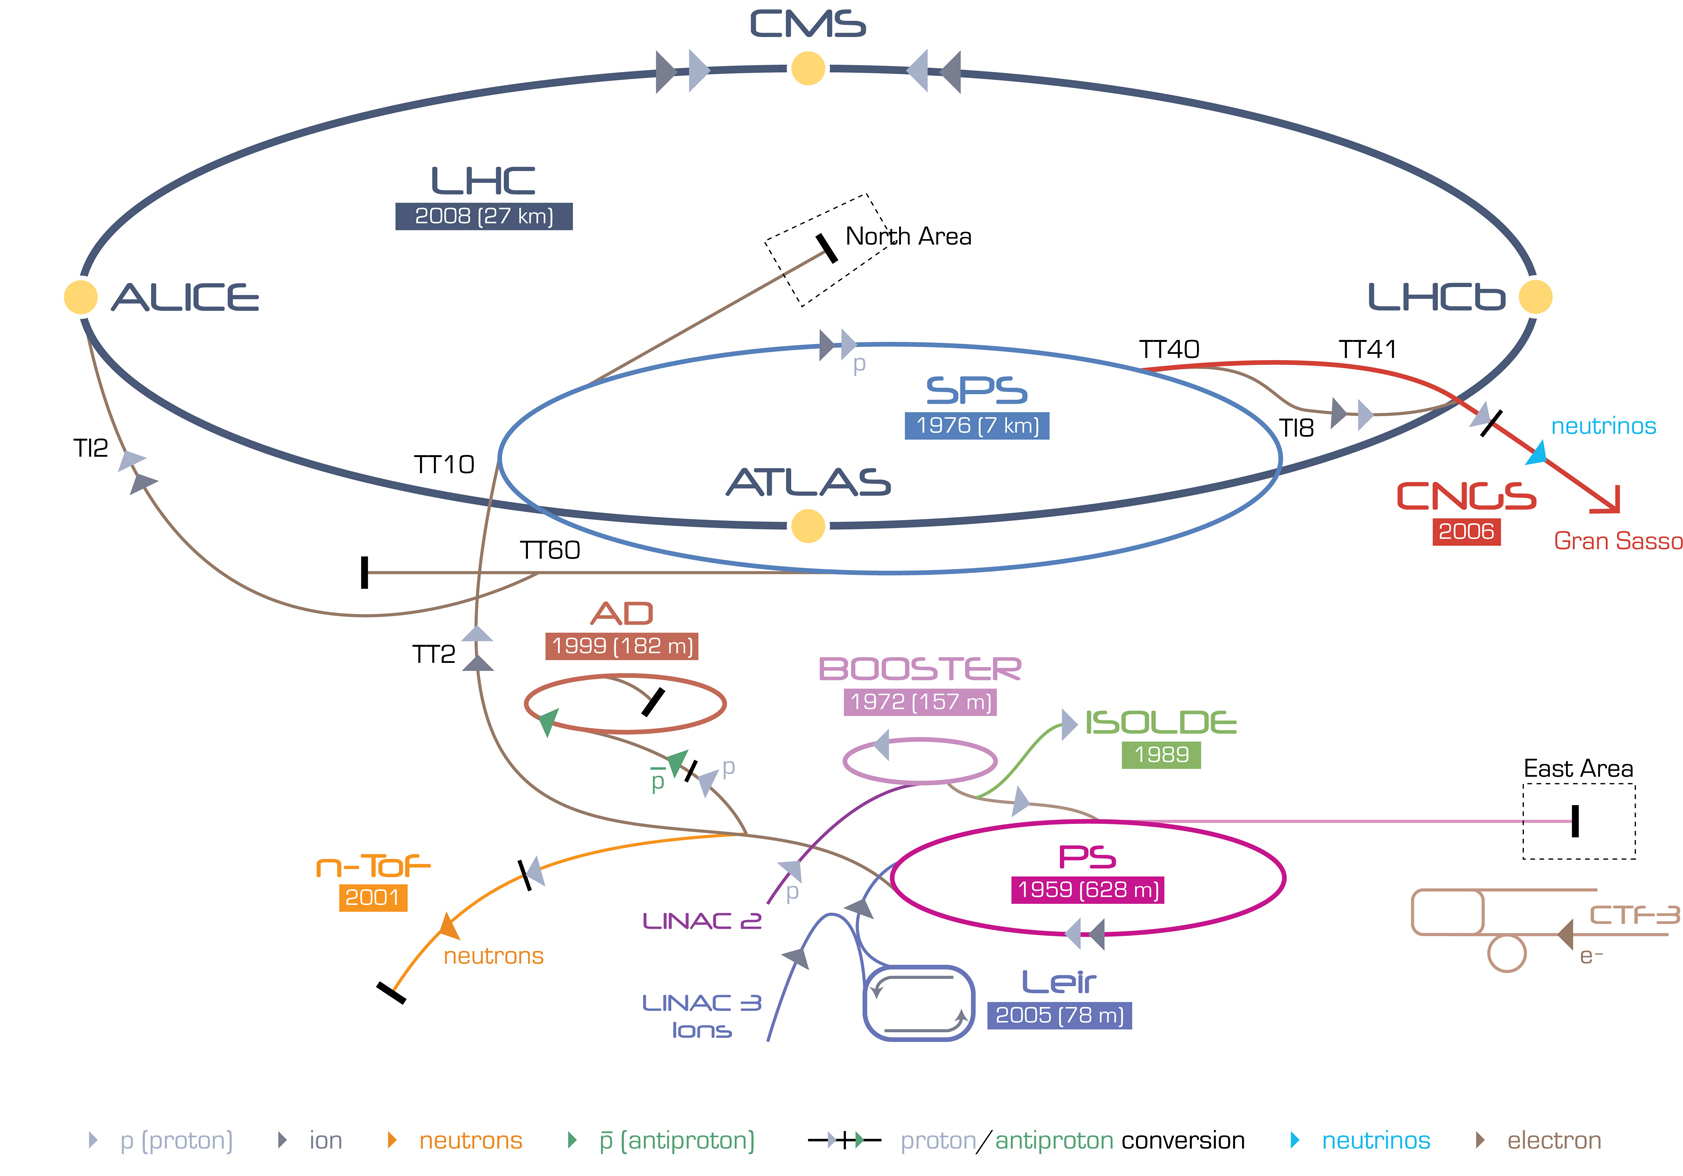
\includegraphics[width=0.65\textwidth,trim=4 4 4 4,clip]
            {Cern-Accelerator-Complex2.jpg}
    \end{center}
\end{frame}

%------------------------------------------------

\begin{frame}
    \frametitle{The Detectors}
    \begin{center}
        \vspace{-1em}
        \includegraphics[width=0.7\textwidth,trim=4 4 4 4,clip]{Atlas.jpg}
    \end{center}
\end{frame}

%------------------------------------------------

\begin{frame}
    \frametitle{Data Flow}
    \begin{center}
        \vspace{-1em}
        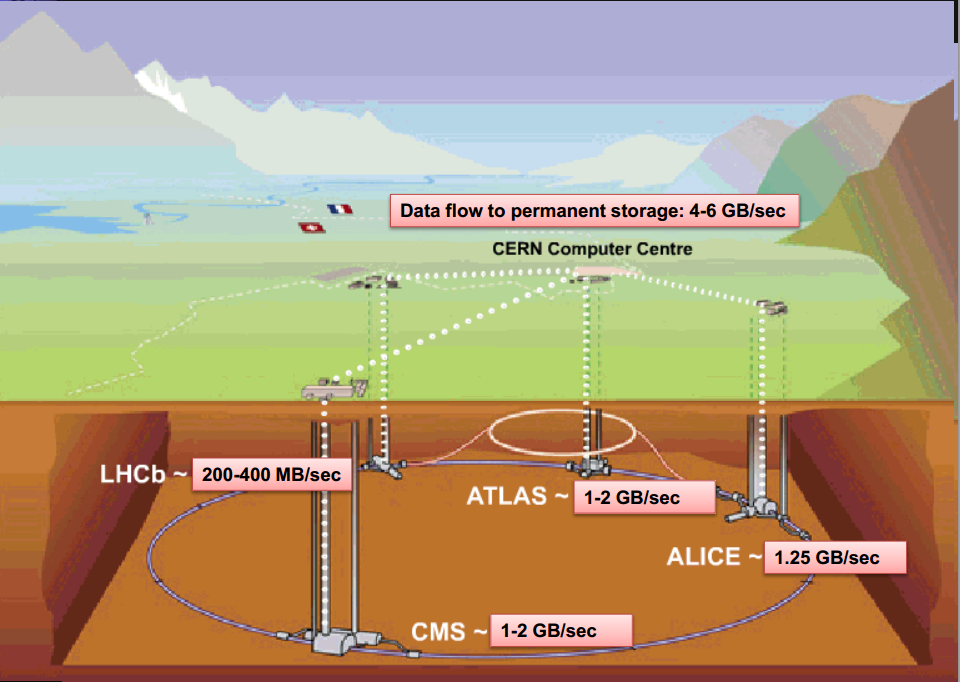
\includegraphics[width=0.65\textwidth,trim=4 4 4 4,clip]
            {LHC_DataFlow.png}
    \end{center}
\end{frame}

%------------------------------------------------

\subsection{Datacenters Overview}
\begin{frame}
    \frametitle{Datacenters in Numbers}
    \begin{minipage}[t]{0.95\textwidth}
        \begin{columns}[T]
            \begin{column}{0.5\textwidth}
                Two datacenters:
                \begin{itemize}
                    \item Budapest
                    \item Geneva
                \end{itemize}
                Two dedicated links:
                \begin{itemize}
                    \item 2 x 100Gbps
                \end{itemize}
                \vspace{0.1in} 
                The number of resources is growing year by year.
                As today:
                \begin{itemize}
                    \item 15k servers
                    \item 100PB on tape
                    \item 200PB on disk
                \end{itemize}
            \end{column}
            \begin{column}{0.5\textwidth}
                \vspace{0.2in} 
                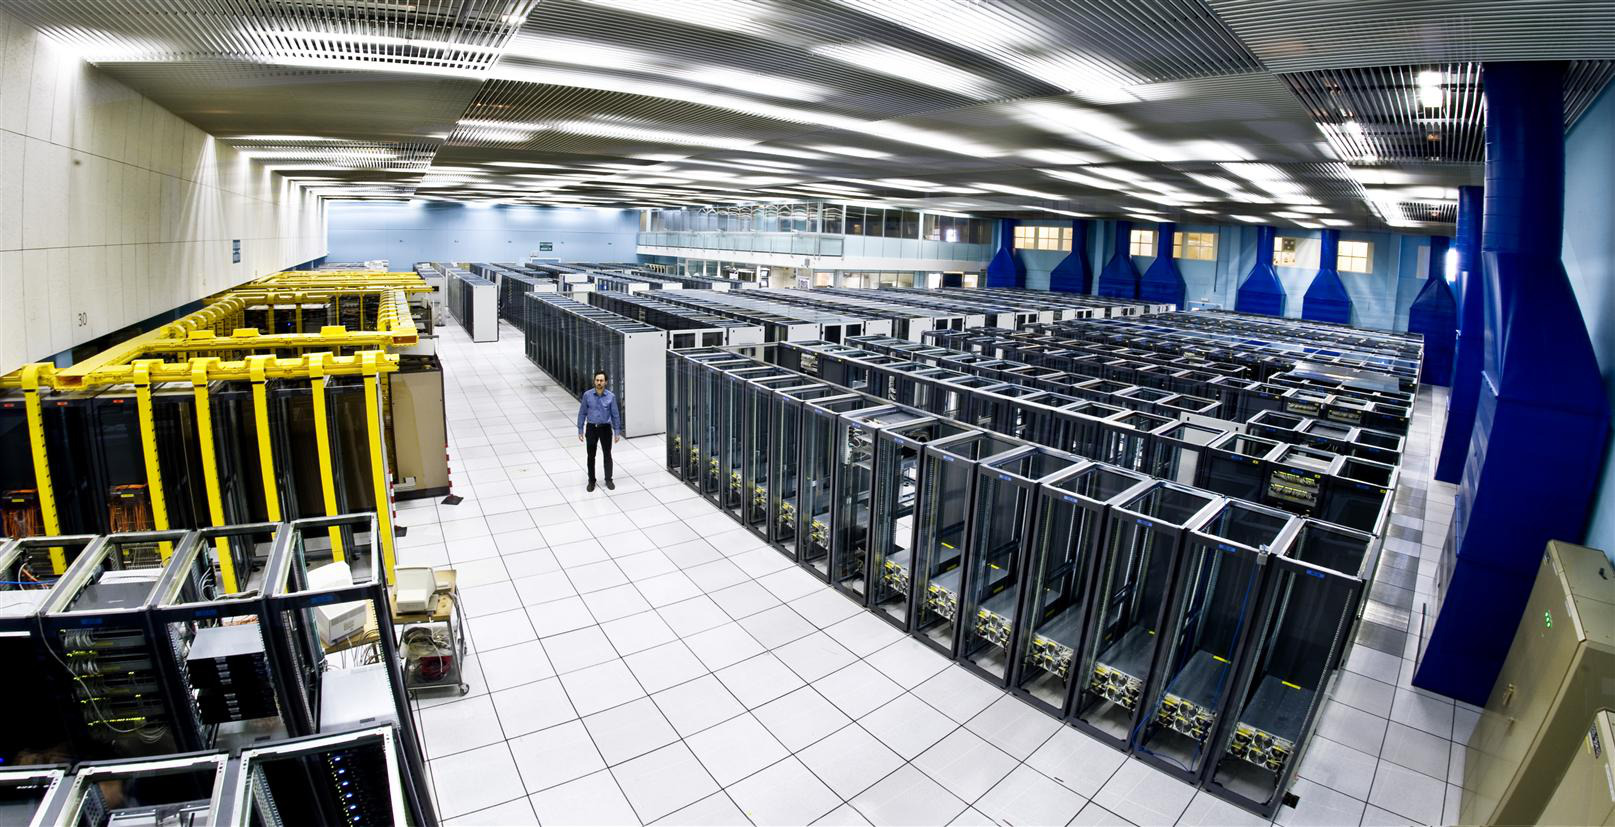
\includegraphics[width=1.1\textwidth]{DC_overview.png}
            \end{column}
        \end{columns}
    \end{minipage}
\end{frame}

%------------------------------------------------

\begin{frame}
    \frametitle{Going Agile}
    \begin{minipage}[t]{0.95\textwidth}
        \begin{columns}
            \begin{column}{0.8\textwidth}
                Requirements started to grow
                \begin{itemize}
                    \item Agile approach was needed
                \end{itemize}
                Since a few years we started using Openstack to deploy virtual 
                machines for our users and Puppet to configure the services 
            \end{column}
            \begin{column}{0.2\textwidth}
                
\includegraphics[width=0.9\textwidth]{openstack-logo512.png}
            \end{column}
        \end{columns}
    \end{minipage}
    \vspace{\belowdisplayskip}
    \vspace{\belowdisplayskip}
    \begin{minipage}[t]{0.95\textwidth}
        \begin{center}
        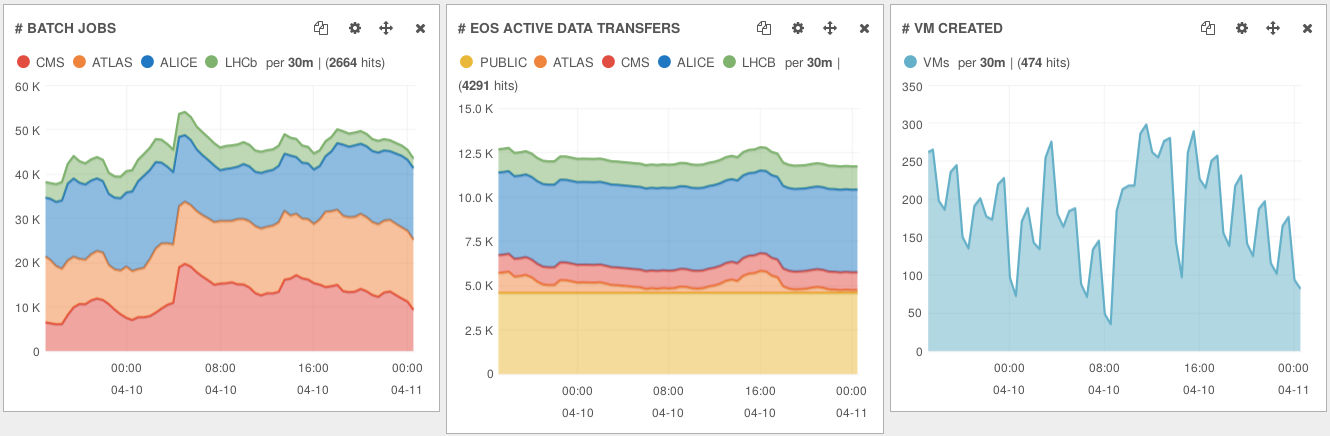
\includegraphics[width=0.83\textwidth]{Eos-CreatedVm.png}
    \end{center}
    \end{minipage}
\end{frame}

%------------------------------------------------
\section{Puppet @ CERN}
%------------------------------------------------

\subsection{Current Infrastructure}
\begin{frame}
    \frametitle{Our Setup}
    We started using Puppet a few years ago and, since then, 
    things evolved a lot \ldots \\
    \vspace{1em}
    We changed several time the configuration of our puppet masters in order 
    to keep up with the requests and we found out that:
    
    \begin{itemize}
        \item Puppet scales horizontally quite well
        \item The NFS filer underneath \ldots does not
    \end{itemize}
\end{frame}

%------------------------------------------------

\begin{frame}

    \frametitle{Clusters and Pools}
    \begin{minipage}[t]{0.95\textwidth}
        \begin{center}
            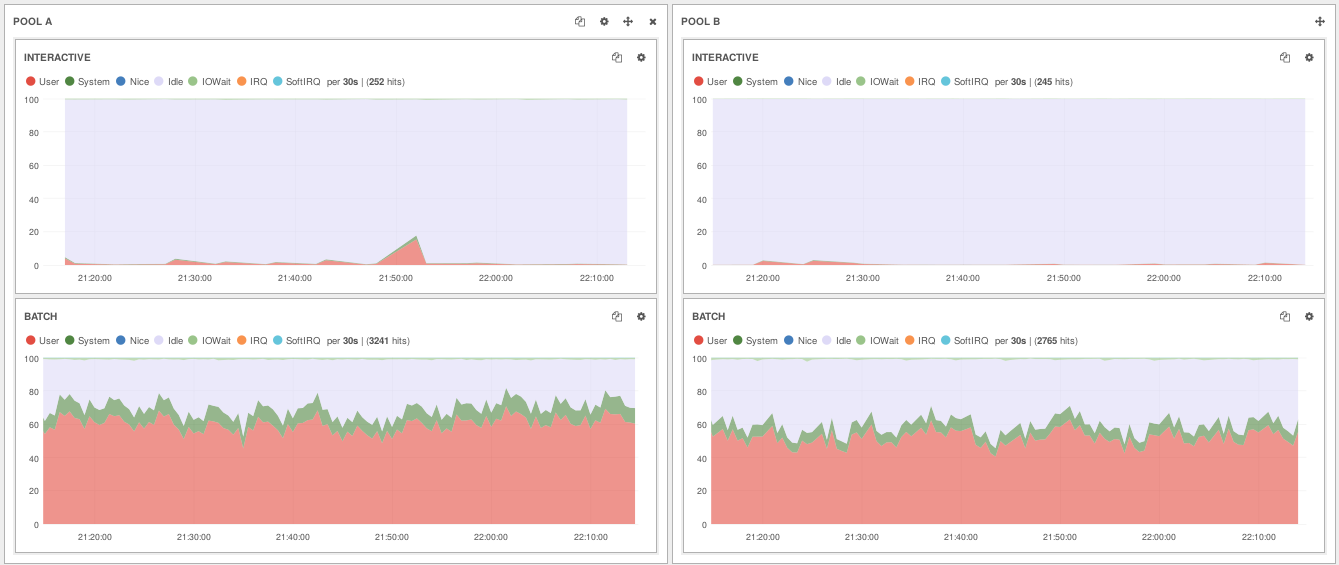
\includegraphics[width=0.85\textwidth]{Puppet_Pools.png}
        \end{center}
    \end{minipage}
    \begin{minipage}[T]{0.95\textwidth}
        \begin{columns}
            \begin{column}{0.5\textwidth}
                \begin{itemize}
                    \item Two Separate Pools
                    \item Machines are assigned to one pool
                \end{itemize}
            \end{column}
            \begin{column}{0.5\textwidth}
                \begin{itemize}
                    \item Batch $\sim 36$ machines
                    \item Interactive $\sim 3$ machines
                \end{itemize}
            \end{column}
        \end{columns}
    \end{minipage}

\end{frame}

%------------------------------------------------

\subsection{Modules, Hostgroups and Environments}
\begin{frame}
    
    \frametitle{Few concepts}
    \begin{itemize}
        \item Modules ($\sim 280$) \\

        The various modules available should be viewed as a library 
        that your hostgroup code can reuse.
        \newline
        \item Hostgroups ($\sim 160$) \\

        Groups of nodes that are part of the same service and have 
        some configurations in common.
        \newline
        \item Environments ($\sim 180$) \\

        Collections of modules and hostgroups at different development levels.
    \end{itemize}

\end{frame}

%------------------------------------------------

\begin{frame}

    \frametitle{Environments allow us to \ldots}

    Environment "production"
        $\rightarrow$ All modules/hg from "master" branch

    Environment "qa"
        $\rightarrow$ All modules/hg from "qa" branch
    \newline 
    \newline 
    Custom environments (for testing purpose):
    \begin{itemize}
        \item Possibility to set a “default” branch
        \item Specify specific branch for one or more modules/hostgroups
    \end{itemize}
    \begin{center}
        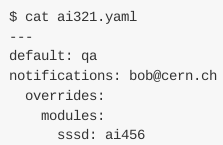
\includegraphics[width=0.35\textwidth]{Env_example.png} \,
        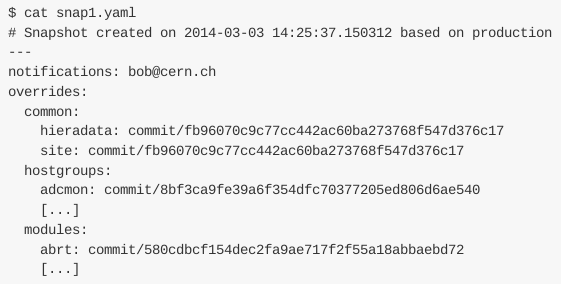
\includegraphics[width=0.45\textwidth]{Env_example_commit.png}
    \end{center}

\end{frame}

%------------------------------------------------
\section{Configuration Management}
%------------------------------------------------

\subsection{Managing Changes}
\begin{frame}
    \frametitle{Manage changes}
    \begin{minipage}[T]{0.95\textwidth}
        \begin{columns}
            \begin{column}{0.5\textwidth}
                Three important concepts:
                \begin{itemize}
                    \item Modules
                    \item Hostgroups
                    \item Environments
                \end{itemize}
                A configuration change has to be approved through 
                a request in Jira.
                \newline
                \newline
                Every git repo has at least two branches:
                \begin{itemize}
                    \item master
                    \item qa
                \end{itemize}
            \end{column}
            \begin{column}{0.5\textwidth}
                \begin{center}
                    
\includegraphics[width=0.85\textwidth]{Git-Logo-1788C.png}
                    \\[2em]
                    \includegraphics[width=0.85\textwidth]
                        {{800px-JIRA_logo.svg}.png}
                \end{center}
            \end{column}
        \end{columns}
    \end{minipage}

\end{frame}

%------------------------------------------------

\begin{frame}
    \frametitle{Puppet Run}
    \vspace{-1em}
    \begin{center}
        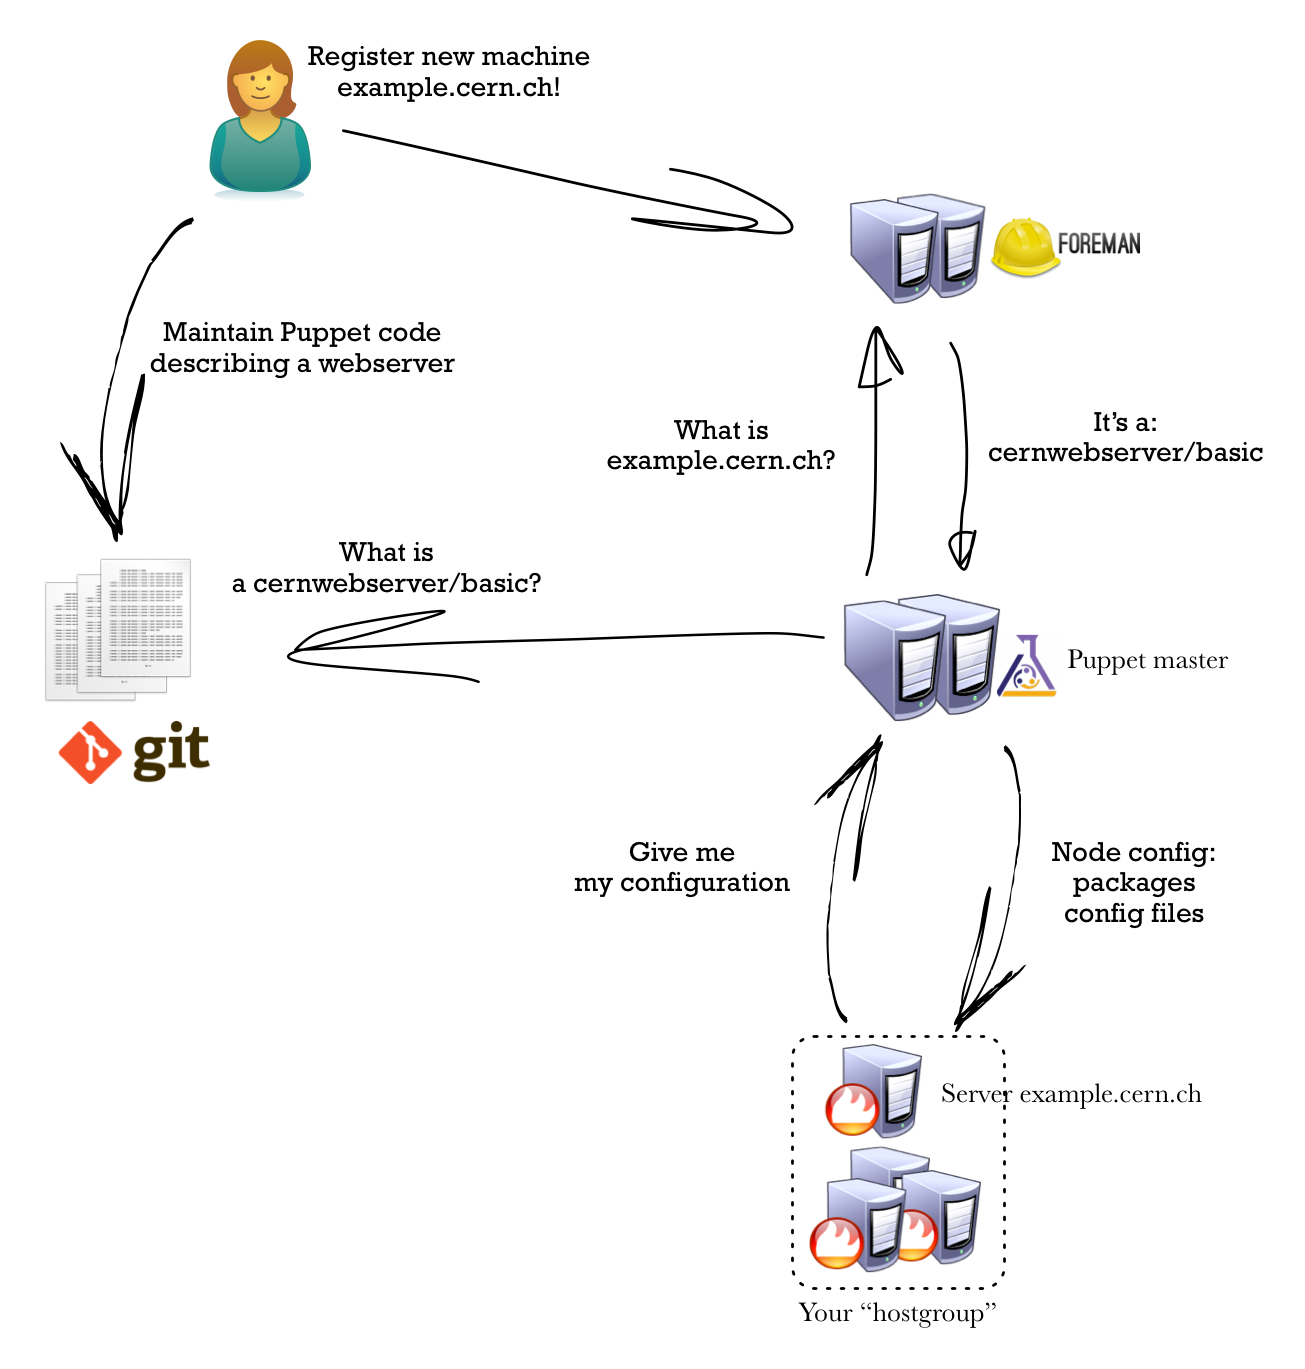
\includegraphics[width=0.5\textwidth]{puppetrun3.png}
    \end{center}
\end{frame}

%------------------------------------------------

\subsection{Tools}
\begin{frame}
    \frametitle{Jens}
    Jens creates Puppet environments for the Puppet Masters
    \begin{itemize}
        \item Using repository metadata and a list of environments definitions
        \item Allows dynamic environments and isolates puppet code 
            for different services
    \end{itemize}
    \vspace{2em}
    Has recently been opensourced on GitHub: \\
    \vspace{1em}
    \begin{center}
        \textbf{https://github.com/cernops/jens} \\
    \end{center}
    \vspace{1em}
    Useful for those running different services under the 
    same puppet infrastructure
\end{frame}

%------------------------------------------------

\begin{frame}
    \frametitle{Configuration Change Process}
    Configuration change process:
    \begin{itemize}
        \item Modify a module on feature branch
        \item Create a custom env and test the module
        \item Open a ticket on Jira and announce the change
        \item Merge to qa
        \item After one week, merge to production
    \end{itemize} \\[2em]

    Service managers use the same module for different services: we need to 
    be sure that all the service managers are happy with the change before 
    merging it to production.
\end{frame}

%------------------------------------------------

\begin{frame}
    \frametitle{Jenkins and Continuous Integration process}
    \begin{minipage}[T]{0.95\textwidth}
        \begin{columns}
            \begin{column}{0.5\textwidth}
                \begin{itemize}
                    \item Machines are built and tested before merging a 
                        change to production
                    \item More automation, less manual work
                    \item Still work in progress, but looks promising
                \end{itemize}
            \end{column}
            \begin{column}{0.5\textwidth}
                \begin{center}
                    
\includegraphics[width=0.5\textwidth]{Jenkins_headshot.png}
                \end{center}
            \end{column}
        \end{columns}
    \end{minipage}
\end{frame}

%------------------------------------------------

\begin{frame}
    \frametitle{Dashboard}
        \begin{center}
            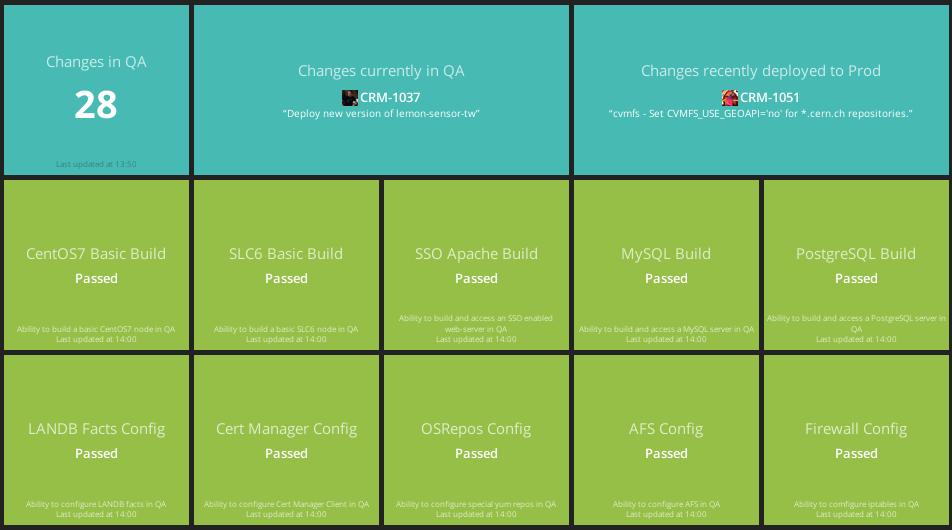
\includegraphics[width=0.8\textwidth]{CI-dashboard.png}
        \end{center}
\end{frame}

%------------------------------------------------

\begin{frame}
    \frametitle{Automating procedures - RunDeck}
    \begin{minipage}[T]{0.95\textwidth}
        \begin{columns}
            \begin{column}{0.5\textwidth}
                \begin{center}
                    
\includegraphics[width=0.7\textwidth]{Rundeck.png}
                \end{center}
            \end{column}
            \begin{column}{0.5\textwidth}
                \begin{itemize}
                    \item Tedious prone-error tasks replaced by executable code
                    \item Handing off operational tasks to others
                    \item Procedures as a list of individual and atomic steps 
                    \item Ability to react to failures
                \end{itemize}
            \end{column}
        \end{columns}
    \end{minipage}
\end{frame}

%------------------------------------------------

\begin{frame}
    \frametitle{Renaming hosts}
    \begin{center}
        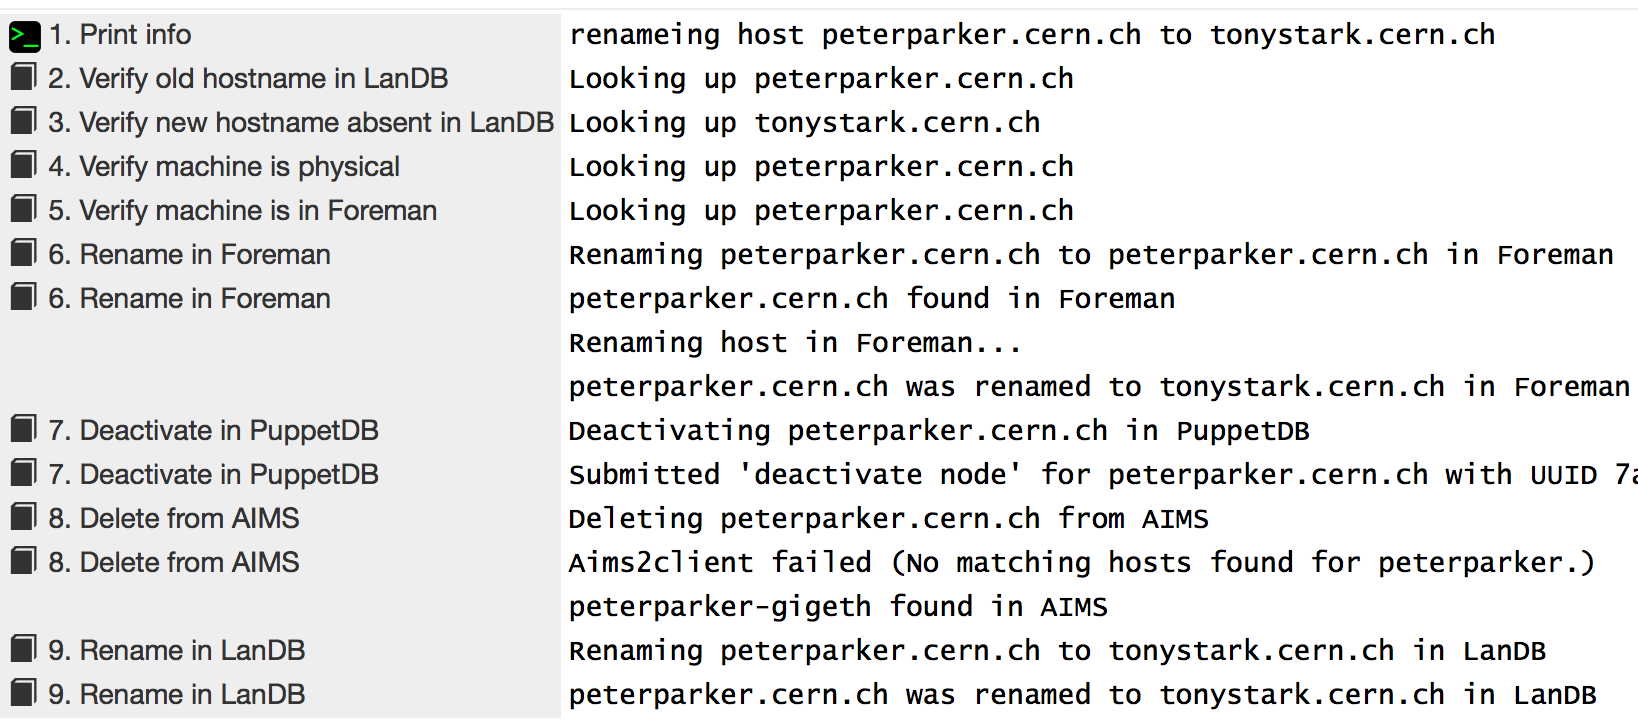
\includegraphics[width=0.9\textwidth]{RunDeck_rename.png}
    \end{center}
\end{frame}

%------------------------------------------------

\begin{frame}
    \frametitle{Mcollective}
    \begin{minipage}[T]{0.95\textwidth}
        \begin{columns}
            \begin{column}{0.5\textwidth}
                Framework for server orchestration and parallel 
                job execution \\[2em]

                Problems in the past with big clusters \\
                $\textgreater$ 3000 nodes \\[2em]

                Latest improvements:
                \begin{itemize}                
                    \item Direct addressing
                    \item New PuppetDB discovery method
                    \item Threaded Mode
                    \item Batched requests
                \end{itemize}
            \end{column}
            \begin{column}{0.5\textwidth}
            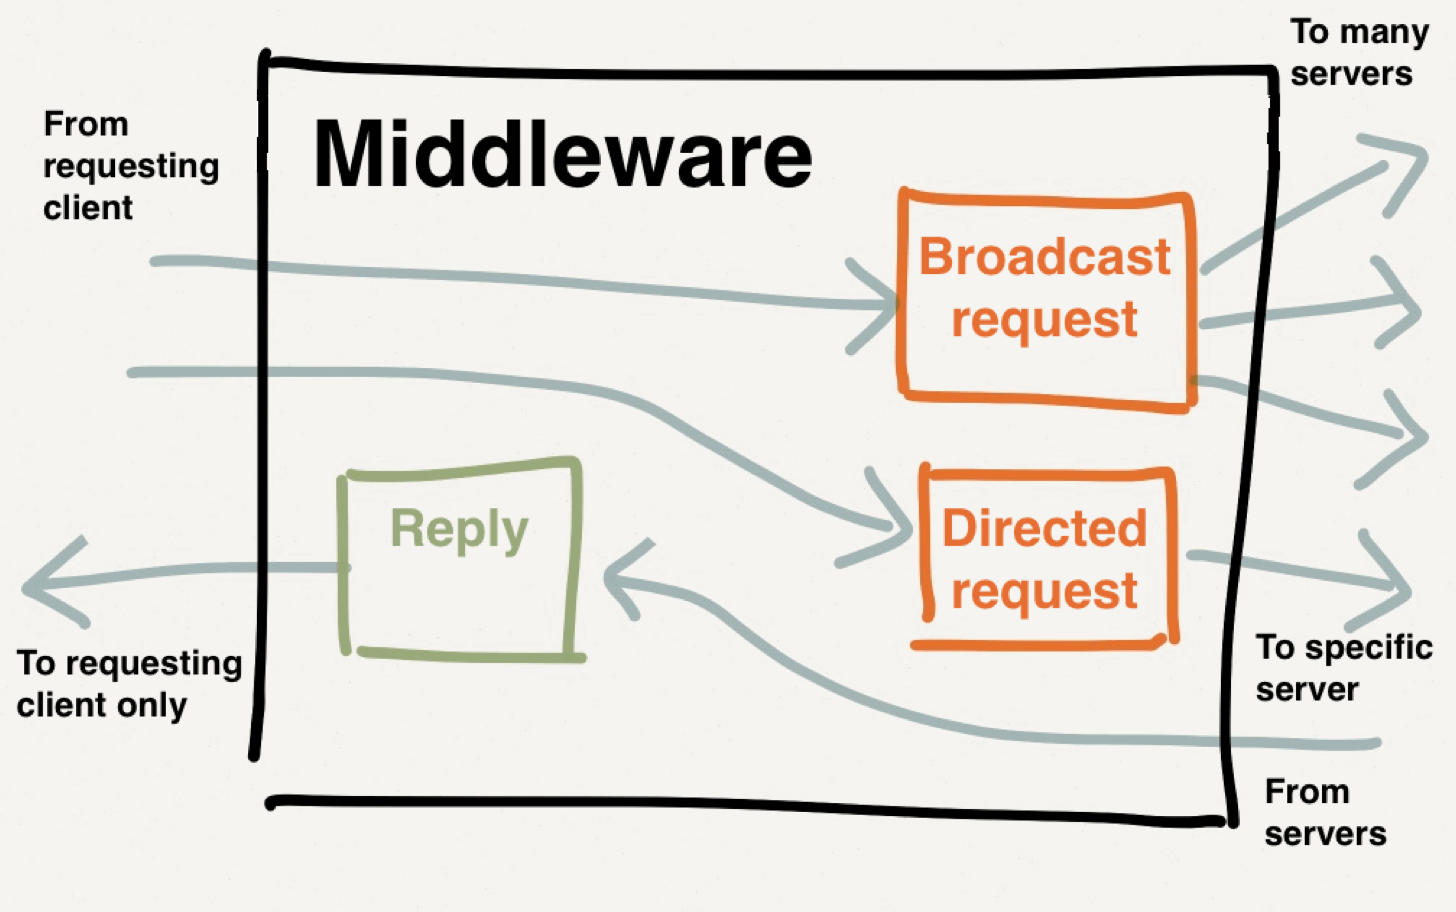
\includegraphics[width=1.1\textwidth]{mco.png}
            \end{column}
        \end{columns}
   \end{minipage} 
\end{frame}

%------------------------------------------------

\begin{frame}
    \frametitle{Configuration Drifts}
    \begin{minipage}[t]{0.95\textwidth}
        Configuration drifts started to be a problem:
        \begin{itemize}
            \item Out of sync machines
            \item Possibility for service managers to have snapshots
            \item Possibility to “freeze” their environment
       \end{itemize}
       It's not easy to keep all the configuration in sync
    \end{minipage}
    \vspace{\belowdisplayskip}
    \begin{minipage}[t]{0.95\textwidth}
        \begin{center}
            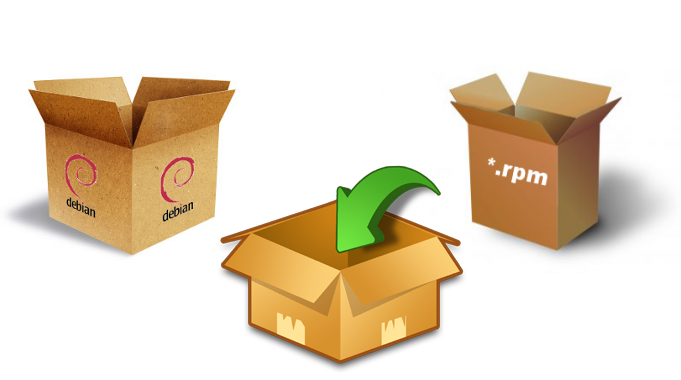
\includegraphics[width=0.5\textwidth]{package.png}
        \end{center}
    \end{minipage}
\end{frame}

%------------------------------------------------

\begin{frame}
    \frametitle{Package Inventory}
    \begin{minipage}[t]{0.95\textwidth}
        Centralized service for package inventory:
        \begin{itemize}
            \item Using Elasticsearch
            \item Queryable using Cli
            \item Compare a set of hosts
            \item Reports differences and misalignments
            \item Package History
        \end{itemize}
    \end{minipage}
    \vspace{\belowdisplayskip}
    \vspace{\belowdisplayskip}
    \begin{minipage}[t]{0.95\textwidth}
        \begin{center}
            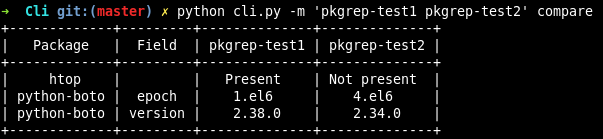
\includegraphics[width=0.8\textwidth]{pkginv_demo.png}
        \end{center}
    \end{minipage}

\end{frame}

%------------------------------------------------
\section{Conclusions}
%------------------------------------------------

\begin{frame}
    \frametitle{Conclusions}
    Moving from a traditional infrastructure to an Agile one allowed us to:
    \begin{itemize}
        \item Optimize our resources
        \item Speed up the development cycle
        \item Reduce interventions time
        \item Have more free time :)
    \end{itemize}
\end{frame}

%------------------------------------------------

\begin{frame}
    \frametitle{Conclusions}
    Puppet gives us the right combination between elasticity and efficiency \\

    \begin{itemize}
        \item Big community
        \item Active development
        \item Highly customizable
    \end{itemize}

\end{frame}

%------------------------------------------------

\cernSplashBlue

\end{document} 
